\chapter{Thermal Energy and Solids}
\label{chapter:thermal_energy}

\section*{Objectives}
\begin{objectives}

\item For a molecular system, be able to distinguish mechanical energy and
  thermal energy.

\item Given the molecular weight, density, and Young's modulus of a solid,
 derive the appropriate mass, equilibrium length, and spring constant
of the ball-spring model.

\item Use the ball-spring model to describe properties of a solid, including
its molar specific heat and speed of sound.

\item Given two substances, identify the conditions for when their
  thermal energies will change due to heat flow and when they are in
  thermal equilibrium.  Be able to quantitatively relate the heat flow
  to a temperature change.

\end{objectives}

\section{Introduction}

In our everyday lives we experience many examples where mechanical
energy is not conserved: brakes slow down a car, a bouncing superball
returns to a lower height than it started from, and blow darts slide
to a stop along the corridors of Bucknell residence halls.  Because
friction takes mechanical energy away from an object, historically
it was not at all obvious that energy should be conserved.
But some physicists in the 19th century noticed that when friction
acts to slow an object and take away some mechanical energy, the
object invariably becomes hotter.  This suggested that temperature is
connected to some kind of internal energy of the object --- let's call
it {\it thermal energy} --- and that friction has acted to convert
some of the object's mechanical energy to this thermal energy.
Careful experiments by Joule and others confirmed the hypothesis that
total energy is conserved even when mechanical energy is gained or
lost, and now energy conservation is one of the most fundamental
principles in physics.

But what is thermal energy?  As we shall see, it is nothing more than
the kinetic and potential energy of the individual molecules that make
up the objects in our everyday world.  In this unit we will begin by
distinguishing mechanical energy from thermal energy.

\section{Thermal Kinetic Energy}

First, let's consider molecular kinetic energy.  Consider a set of $N$
molecules, each with the same mass $m$, with velocities $\vec v_1$,
$\vec v_2$, \dots, $\vec v_N$.  We will show that the kinetic energy
associated with these moving molecules can be separated into
mechanical kinetic energy and thermal kinetic energy.  The first step
is to calculate the motion of what is called the {\it center of mass.}
At some particular instant in time, the positions of each particle are
given by the vectors $\vec r_1$, $\vec r_2$, \dots, $\vec r_N$.  The
location of the center of mass, denoted by the vector $\vec r_{cm}$,
is the average of these positions
\begin{equation}
\vec r_{cm} = \frac{1}{N}(\vec r_1 + \vec r_2 + \dots + \vec r_N).
\end{equation}
Taking a time derivative of this equation gives
\begin{equation}
\vec v_{cm} = \frac{d\vec r_{cm}}{dt} =
\frac{1}{N}(\vec v_1 + \vec v_2 + \dots + \vec v_N),
\end{equation}
so the center of mass velocity is simply the average velocity (in this
simplified case of equal masses).  

For a rigid object, like a solid, the velocity of the center of mass
is simply the velocity of the object.  If the center of mass velocity
of some object is zero, then that object, viewed macroscopically, is at
rest.  A ball sitting on a table has a stationary center of mass, and
therefore no mechanical kinetic energy.  However, the individual
molecules of the ball are certainly not at rest and do have kinetic
energy.  The motion appears random, with molecules moving in every
direction; some molecules moving faster and some slower.  It is this
molecular kinetic energy which we identify as thermal
energy.\footnote{For simplicity, we are excluding the possibility of
  rotations.}

\boxittext{The thermal kinetic energy of an object is simply the
  molecular kinetic energy when the center of mass is at
  rest.}

What about the case where the center of mass is moving?  For example,
if the ball is not sitting on the table but rather flying through the
air.  It is still possible to identify the thermal kinetic energy,
because there is always some co-moving reference frame in which the
ball is at rest.  The molecular motion as viewed in that
frame will again be the thermal kinetic energy.

But nevertheless we may ask if
it is possible to identify the thermal kinetic energy in a frame where
the ball is moving.  And indeed, it is possible.  The velocity $\vec
v_i$ of the $i$th molecule can be written as a sum of the center of
mass velocity $\vec v_{cm}$ and the velocity of the particle relative
to the center of mass $\vec v_{i,rel}$.  That is, $\vec v_i = \vec
v_{cm} + \vec v_{i,rel}$.  Then the total kinetic energy is the sum
over all particles:
\begin{align}
K_\text{total} &=
{\textstyle\frac{1}{2}}\sum_i m (\vec v_{cm}+\vec v_{i,rel})\cdot  
(\vec v_{cm}+\vec v_{i,rel}) \nonumber\\
&= {\textstyle\frac{1}{2}}\sum_i m\, v_{cm}^2 
+\sum_i m\,\vec v_{cm}\cdot \vec v_{i,rel}
+ {\textstyle\frac{1}{2}}\sum_i m\, v_{i,rel}^2.
\label{eq:kinetic_energy}
\end{align}
Note that $\vec v_{cm}$ is the same for all particles, so it can be
brought outside the sum over particles.  Then the first term becomes
\begin{equation}
{\textstyle\frac{1}{2}}\sum_i m\, v_{cm}^2  = {\textstyle\frac{1}{2}}v_{cm}^2
\sum_i m = {\textstyle\frac{1}{2}}Mv_{cm}^2,
\end{equation}
where $M$ is the total mass of all the particles.  This is exactly the
mechanical kinetic energy we have already encountered.  The second
term can be written as
\begin{equation}
m\vec v_{cm} \cdot \left( \sum \vec v_{i,rel}\right). 
\end{equation}
Since $\vec v_{i,rel}$ is the particle velocity relative to the center
of mass frame, the sum $\sum \vec v_{i,rel}=0$, and this term
vanishes.  The last term in Eq.~(\ref{eq:kinetic_energy}) is just the
total kinetic energy measured in a frame moving with the center of
mass, which is the thermal kinetic energy.  Putting this all together,
\begin{equation}
K = K_\text{mech} + K_\text{therm},
\end{equation}
thus the kinetic energy divides cleanly into mechanical and thermal
kinetic energy.

\section{Thermal Potential Energy}

Thermal energy is not just kinetic, but also involves potential
energy.  Mole\-cules exert forces on each other, pushing and
pulling.\footnote{The origin of these forces is the electric force
  interactions between the charges of the atoms combined with quantum
  mechanics, which governs the location of the charges.  Both of these
  topics will be covered in PHYS 212.}  These forces are conservative,
so there is a potential energy associated with each pair of molecules.
To understand this potential energy, we must first consider the force
between an isolated pair of molecules.  There are three distinct
regimes, depending on how far apart the two molecules are.
\begin{itemize}
\item When the molecules are closer than a molecular diameter, they
exert a strong repulsive force on each other.
\item When the molecules are within a few molecular diameters, they
exert attractive forces on each other.
\item When the molecules are more than a few molecular diameters away
from each other, the force becomes negligibly small.
\end{itemize}

This behavior is captured by what is called the {\it pair
  potential\/}, shown in Fig.~\ref{fig:pair_potential}, which is the
potential energy $U_\text{pair}(r)$ due to a pair of molecules
separated by a distance $r$.  The diagram illustrates the three
regions.  Notice that at a separation $r=d$, where $d$ is the
molecular diameter, there is an equilibrium point dividing the regions
of attractive and repulsive forces.

As we shall see in the next two chapters, this pair potential explains
the existence of solid, liquid, and gas phases, and many details of
the phases and of the transitions between the phases.  It is one of
the remarkable triumphs of the atomic theory of matter that so much
behavior can be explained by such a simple model of the forces between
atoms!

In principle, the {\it system} potential energy for a system of $N$
molecules contains the pair potential energy for every single pairing
of the molecules.  This is a very large number of pairs!  Fortunately,
only those molecules which are immediate neighbors are close enough to
have an appreciable force and potential energy, so we only need to
consider the potential energy due to neighboring molecules.

\begin{figure}
\begin{center}
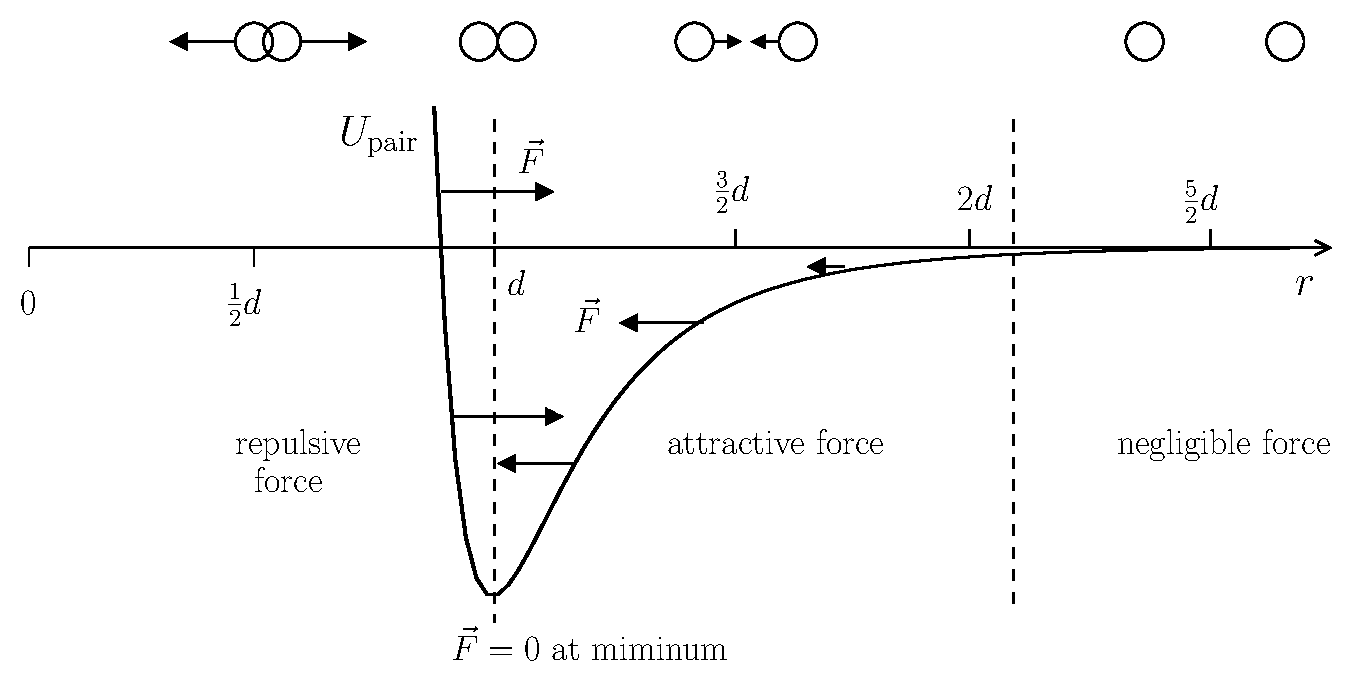
\includegraphics[width=5in]{thermal_energy_and_solids/pair_potential.eps}
\caption{The pair potential energy $U_\text{pair}$ as a function of $r$, the
  separation between the pair of molecules.  The dashed lines separate
  the regions of repulsive force, attractive force, and no force.  At
  separation $r=d$ the pair is in equilibrium, which defines the
  molecular diameter.}
\label{fig:pair_potential}
\end{center}
\end{figure}

What about other sources of potential energy besides the
intermolecular forces?  For example, gravitational potential energy.
When a ball is thrown upwards, the gravitational potential energy of
each molecule increases.  But the height of each molecule is increased
by the same amount that the height of the center of mass is increased.
Therefore this change in potential energy has the form
\begin{equation}
\Delta U_\text{grav} = M_\text{object} g\Delta y_{cm},
\end{equation}
where $M_\text{object}$ is again the total mass of the object.  This
is the familiar mechanical potential energy.  Therefore, gravitational
potential energy is always part of the mechanical energy, whereas the
molecular interaction energy makes up the thermal potential energy.

In summary, here is the big picture for thermal energy:
\begin{itemize}
\item For both potential energy and kinetic energy, it is the
  `organized' motion that makes up the {\it mechanical energy}, such as
  all molecules increasing their height together or all molecules
  having a net alignment of their velocities.
\item The remaining disorganized motion, such as the wiggling of the
  mole\-cules and their individual pushes and pulls on each other,
  corresponds to the {\it thermal energy}.
\item Friction is an agent that takes organized motion and
  disorganizes it, taking away mechanical energy and increasing thermal
  energy.
\item Going the other way --- taking away thermal energy and
  increasing mechanical energy --- is more difficult, since molecules
  are not likely to spontaneously start moving together.
  Nevertheless, we can capture some amount of thermal energy and
  convert it to mechanical energy with a device called a heat engine,
  which is the topic of Supplementary Reading Chapter
  \ref{chapter:heat_engines}.
\end{itemize}

\section{The Solid State}

\label{section:the_solid_state}

Molecules interacting via the pair potential can be solids, liquids,
or gases.  The remainder of this chapter is concerned with the thermal
energy of the solid state, while liquid and gas states will be
presented in Chapter \ref{chapter:liquids_and_gases}.


Most inorganic solids are crystalline, which means the molecules are
arranged in a symmetric way, such as a cubic lattice.  (Organic
  solids instead are constructed from long carbon chains.)  In this
lattice, each pair of neighboring molecules is separated by roughly
the equilibrium distance, that is, the minimum of the pair potential
well, and only makes small excursions from this location.  As
illustrated in Fig.~\ref{fig:pair_potential_spring}, the pair
potential in this region is identical to a parabolic potential.  We
have previously encountered a parabolic potential energy curve as the
potential energy for a mass on a spring.  Evidently, as long as the
molecules in a solid are not deviating significantly from their
equilibrium position, we may regard their interactions with their
nearest neighbors as equivalent to being attached by a spring.

\boxittext{{\sc Checkpoint:} What is the main difference between the pair
  potential and the spring potential?  What would I need to do to a
  pair of molecules to see this difference?  (Push together?  Pull
  apart?  How far?) }

\begin{figure}
\begin{center}
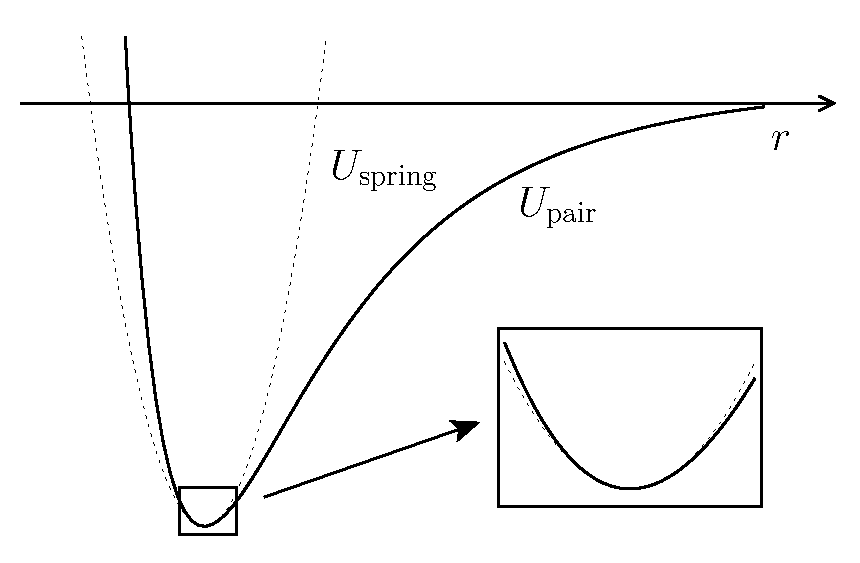
\includegraphics[width=3.5in]{thermal_energy_and_solids/pair_potential_spring.eps}
\caption{The solid curve is the pair potential $U_\text{pair}$ as a
  function of separation $r$.  The dashed line is the spring potential
  $U_\text{spring}$ with the spring constant $k_{sp}$ chosen to match
  $U_\text{pair}$ near the minimum.  The inset shows the match.}
\label{fig:pair_potential_spring}
\end{center}
\end{figure}


This leads to what we call the {\it ball-spring\/} model of a solid:
the molecules are balls of mass $m$, they are connected by springs of
spring constant $k_{sp}$, and the springs have an equilibrium length
of $d$.  This model is illustrated in Fig.~\ref{fig:ball-spring}.  We
may think of the spring constant as determining the bond strength and
the equilibrium length $d$ as the bond length.  These three parameters
($m$, $d$, and $k_{sp}$) define the model, and we shall see that for
many solids determining these parameters describes much of the
behavior of the solid.

One may imagine packing the molecules together in different ways.  The
arrangement illustrated in Fig.~\ref{fig:ball-spring}, is called a
{\it simple cubic} lattice.  In fact, most solids are packed
differently, for example, in the way a grocer would stack oranges
(which is called a {\it face-centered cubic} lattice).  Fortunately,
this distinction has little impact on the quantities we will study, so
we will stick with the simple cubic lattice.

\begin{figure}
\begin{center}
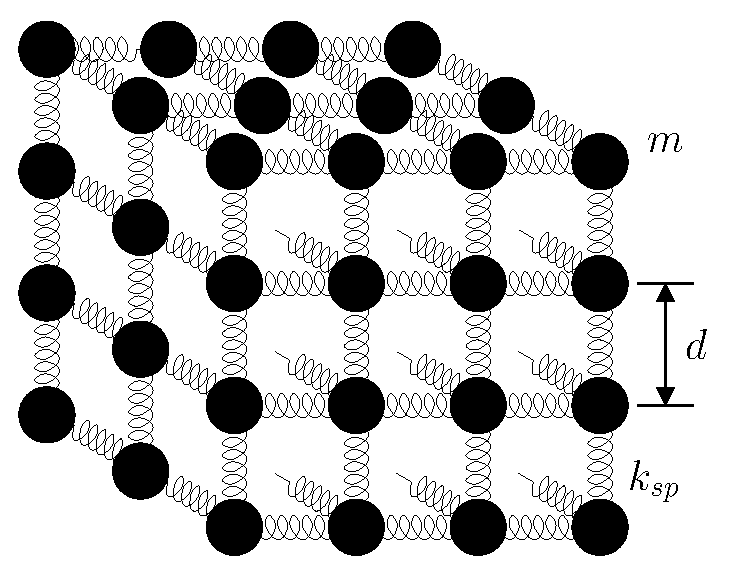
\includegraphics[width=2.5in]{thermal_energy_and_solids/ball-spring.eps}
\caption{The ball-spring model of a solid.}
\label{fig:ball-spring}
\end{center}
\end{figure}

Given the properties of some solid, how are the ball-spring model
parameters determined?  Let's derive these for a specific case, namely
copper.  Molecular properties, such as mass, are usually not specified
for a single molecule, but rather for a {\it mole}.  One mole equals
Avogadro's number
\begin{equation}
N_A=6.02\times 10^{23}
\end{equation} 
of molecules.  Avogadro's number is chosen so that roughly one mole of
protons has a mass of one gram.  The precise definition is that one
mole of carbon atoms has a mass of $12\units{g}$.  The mass of one mole
of a material would logically be called the molar mass, but instead it
is usually called the {\it molecular weight}.\footnote{It's not our fault.}

One mole of copper has mass $64\units{g}$, so we may conclude that a
single molecule of copper (the ball in our model) has mass
\begin{equation}
m_\text{Cu} = \frac{64\units{g}}{6.02\times 10^{23}} = 1.06\times
10^{-22}\units{g}.
\end{equation}
This is the first of our three parameters.

Next, we can get the equilibrium spacing $d$ between the molecules by
knowing the density of copper, which is $8.94\units{g/cm$^3$}$.  
In Fig.~\ref{fig:ball-spring-volume} shows that each molecule of copper
occupies its own cubical region with volume $d^3$.
We can relate the density $\rho$ of the solid to the mass per volume
of a unit cell.  That is,
\begin{equation}
\rho = \frac{\text{mass}}{\text{volume}} = \frac{m}{d^3} 
  \qquad \Rightarrow\qquad d =
\left(\frac{m}{\rho}\right)^{1/3}.
\end{equation}
For copper this gives
\begin{equation}
d_\text{Cu} = \left(\frac{m_\text{Cu}}{\rho_\text{Cu}}\right)^{1/3}
 =  \left(\frac{1.06\times
     10^{-22}\units{g}}{8.94\units{g/cm$^3$}}\right)^{1/3}
 = 2.28\times 10^{-8}\units{cm},
\end{equation}
or equivalently, $2.28\times 10^{-10}\units{m}$.
And so we have the second parameter.

%Next, we can get the equilibrium spacing between the molecules by
%knowing the density of copper, which is $8.94\units{g/cm$^3$}$.  How
%many copper molecules are in a cubic centimeter of copper?    We can 
%calculate this as follows:
%\begin{equation}
%\frac{8.94\units{g}}{64\units{g/mole}} = 0.139 \units{moles}
% = 8.41\times 10^{22} \units{molecules},
%\end{equation}
%where Avogadro's number was used to convert moles to molecules.  The
%cubic centimeter of volume is divided equally among this number of
%molecules so the volume per molecule is
%\begin{equation}
%\frac{1 \units{cm$^3$}}{8.41\times 10^{22}\units{molecules}}
% = 1.19\times 10^{-23}\units{cm$^3$}.
%\end{equation}
%
%The volume for a single molecule can be pictured as a cube of length
%$d$, where $d$ is the bond length (see
%Fig.~\ref{fig:ball-spring-volume}).  Since the volume of a cube is
%$V=d^3$, the bond length is obtained from $d=V^{1/3}$, or
%\begin{equation}
%d = (1.19\times 10^{-23}\units{cm$^3$})^{1/3} = 2.28\times 10^{-8}\units{cm}
% = 2.28\times 10^{-10}\units{m}.
%\end{equation}
%And so we have the second parameter.

\begin{figure}
\begin{center}
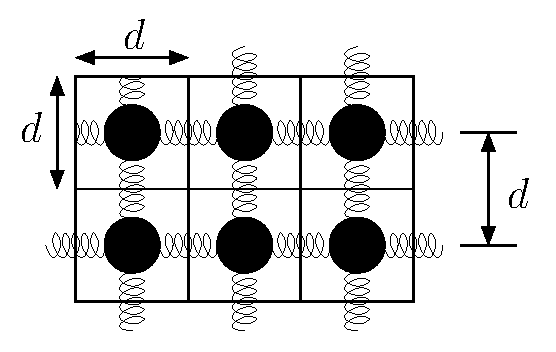
\includegraphics[width=2in]{thermal_energy_and_solids/ball-spring-volume.eps}
\caption{For the ball-spring model with a separation $d$ between the 
balls, the volume per ball is given by a cube of side $d$ (shown here
in two-dimensions).}
\label{fig:ball-spring-volume}
\end{center}
\end{figure}


The final step is to determine the spring constant.  Fortunately, it
is not necessary to try pulling on a single molecule and measuring the
force that it pulls back with.  Rather, a macroscopic chunk of
material can be fixed at one end and pulled on the other, and by
measuring how much the object stretches, the bond spring constant can
be measured.

Imagine a piece of copper wire with cross-sectional area $A$ and
length $L$.  The applied force required to stretch the wire by an amount
$\Delta L$ is given by the following relation:
\begin{equation}
F_\text{app} = \frac{Y A}{L}\Delta L.
\label{eq:force_extension}
\end{equation}
This relation indicates that the amount of stretch $\Delta L$ is
proportional to the amount of force applied; doubling the force will
double the amount of stretch from the equilibrium length.  A larger
cross-sectional area $A$ makes the wire harder to stretch, which
accounts for the factor of $A$ in the numerator.  The longer the wire,
the easier it is to stretch, accounting for the factor of $L$ in the
denominator.  The final parameter $Y$ is called Young's modulus,
and is a property of the material but not dependent on the geometry
of the wire.  For example, Young's modulus for copper is
$Y_{\rm Cu} \approx 130\times 10^9 \units{N/m$^2$}$.  

\begin{example}{Stretching an Extension Cord}
Consider 16 gauge copper wire, commonly used in power cables, which 
has a
cross-sectional area of $1.3\times 10^{-6}\units{m$^2$}$.  How much
force is required to stretch a 2-meter length of wire a distance of
1 centimeter?
\solution
According to Eq.~(\ref{eq:force_extension}), the force is given by
\begin{align}
 F_\text{app} = \frac{Y_{\rm Cu}A}{L}\Delta L &=
 \displaystyle\frac{(130\times 10^9\units{N/m$^2$})(1.3\times
  10^{-6}\units{m$^2$})} {2\units{m}} (0.01\units{m}) \nonumber\\
 &= 845\units{N}.
\end{align}
\end{example} 

Now we need to calculate Young's modulus for the ball-spring model.
Consider a rectangular solid of $N_x \times N_y \times N_z$ molecules.
The object is stretched in the $z$-direction by an applied force $F$,
with a resulting stretch $\Delta L$.  The stretch is shared equally
among each of the $N_z$ springs aligned in the $z$-direction, so each
spring is stretched an amount $\Delta L/N_z$.  The plane of molecules
where the force is applied consists of $N_xN_y$ molecules, each
connected to a spring pulling with force $k_{sp}\Delta L/N_z$.  This
spring force is balancing the applied force, so we can conclude that
\begin{equation}
F_\text{app}= N_xN_y \left(\frac{k_{sp} \Delta L}{N_z}\right).
\end{equation}
If we multiply top and bottom by $d^2$ we can identify the
cross-sectional area $A=(N_x d)(N_y d)$, and the length $L=N_z d$:
\begin{equation}
F_\text{app}=\frac{d^2N_xN_y k_{sp}}{d^2 N_z} \Delta L = \frac{k_{sp}}{d}
\frac{A}{L}\Delta L
\end{equation}
from which we conclude that Young's modulus for the ball-spring model
is
\begin{equation}
Y=\frac{k_{sp}}{d}.
\end{equation}
This can be used to find the spring constant, $k_{sp} = Yd$.  For
example, for copper
\begin{equation}
k_{sp} = (130\times 10^9\units{N/m$^2$})(2.28\times 10^{-10}\units{m})
 = 29.6\units{N/m}.
\end{equation}
In this way, we can find all three ball-spring model parameters from
knowing the molecular weight, the density, and Young's modulus.


\section{Speed of Sound}

How well does this ball-spring picture of a solid work? 
One way to test the model is to study the speed of sound in a
solid.  Sound is a compression wave, much like a compression pulse
sent down a stretched slinky.  If a ball-spring solid is suddenly
struck at one end, how fast does the compression wave travel toward
the other end?  We can almost guess the answer.  The wave ``hops''
from one molecule to its neighbor and each hop moves the wave a
distance $d$.  Since the molecules are harmonic oscillators, the time
it takes for a hop must be related to the period of oscillation $T$,
so we could guess $v_\text{sound} \approx d/T$.  It is not difficult
to do the full calculation for the ball-spring model\footnote{This is
  done in PHYS 221/222.} and find that the answer differs from this
guess by a factor of $2\pi$:
\begin{equation}
v_\text{sound} = \frac{2\pi d}{T} = d\omega  = d\sqrt{\frac{k_{sp}}{m}}
\end{equation}
Thus, the speed of sound in the ball-spring model depends on all three
parameters.  The values we obtained for copper (be careful to use SI
units here!) give
\begin{equation}
 v_\text{sound} = 2.28\times
 10^{-10}\units{m}\sqrt{\frac{29.6\units{N/m}}{1.06\times
     10^{-25}\units{kg}}} = 3810\units{m/s}
\end{equation}
which is exactly the measured value for the speed of sound in copper.
Evidently our ball-spring model works quite well.  You will make more
comparisons in the homework.

\section{Equipartition Theorem}

We began the chapter mentioning that when mechanical energy gets
converted to thermal energy, the temperature increases.  But what is
temperature?  That turns out not to be a simple question and we will
postpone answering it until Chapter \ref{chapter:second_law}.
However, regardless of what it is, we can bring temperature into the
discussion already by taking advantage of the {\it equipartition
  theorem}.

To do this, we must first talk about temperature units.  The Celsius
temperature scale is defined so that water freezes at a temperature of
$0^\circ\units{C}$ and water boils at $100^\circ\units{C}$.  Absolute
zero, the temperature where all molecular motion stops, occurs at
$-273.15^\circ\units{C}$ in the Celsius scale.  

\begin{figure}
\begin{center}
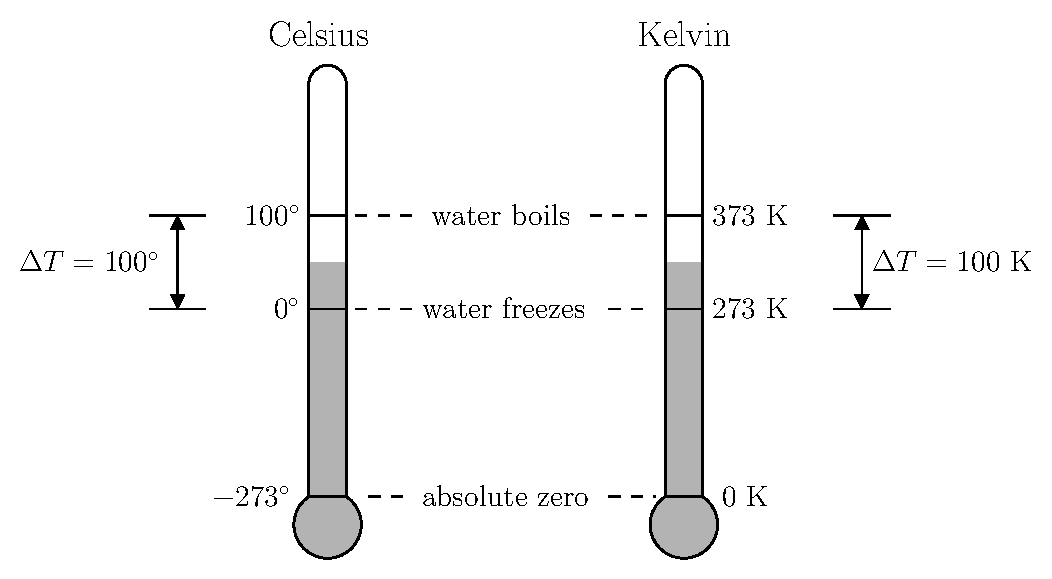
\includegraphics[width=4.5in]{thermal_energy_and_solids/temperature_scales}
\caption{The size of the degree is the same for Celsius and Kelvin
  temperature scales.  They differ by a shift:  $T_K=T_C+273$}
\label{fig:temperature_scales}
\end{center}
\end{figure}

A important variation on the Celsius temperature scale is called the
Kelvin scale, illustrated in Fig.~\ref{fig:temperature_scales}.  The
``size'' of the degree is the same for Kelvin and Celsius, that is, a
change in temperature of $1\units{K}$ is the same as a change in
temperature of $1^\circ\units{C}$.  The boiling temperature of water
is still $100\units{K}$ higher than the freezing temperature. The
difference in the scales is the location of zero: in the Kelvin scale,
absolute zero corresponds to $0\units{K}$, water freezes at
$273\units{K}$ and boils at $373\units{K}$.  To use the equipartition
theorem, we need an absolute temperature scale, that is, one which
goes to zero at absolute zero.  So we must use the Kelvin scale.

And now the theorem:

\boxittext{{\sc Equipartition Theorem:}\\[0.5ex]
  Any term in the energy of a
  molecule that is quadratic, such as $\frac{1}{2}mv_x^2$ or
  $\frac{1}{2}k_{sp}x^2$ or $\frac{1}{2}I\omega^2$, averages to
  $\frac{1}{2}k_BT$.}

This amazing result says that when some $10^{23}$ particles push and pull
and collide with each other, all the messy forces involved will result in
every quadratic energy term averaging to the same value.   It doesn't
matter if the molecule is heavier or lighter, or what the spring
constant is.  It also doesn't matter whether we are talking about
potential energy or translational kinetic energy or rotational kinetic
energy.  As long as the energy is quadratic in the dynamical variable, 
the thermal energy will depend only on $T$ and
Boltzmann's constant,
\begin{equation}
k_B= 1.38\times 10^{-23}\units{J/K},
\end{equation}
which is another constant of nature.  Notice how the units work out:
$k_BT$ is an energy.

\section{Molar Specific Heat}

Now we are prepared to address the question, ``If a certain amount of
thermal energy is added to a system, how much will the temperature
increase?''  For our ball-spring solid, let us make the approximation
that the neighbors of a particular ball remain fixed.  This turns out
to be a reasonable approximation for most solids.  Then the energy
describing that particular ball is
\begin{equation}
E_\text{ball} = {\textstyle\frac{1}{2}}mv_x^2 +
{\textstyle\frac{1}{2}}mv_y^2 + {\textstyle\frac{1}{2}}mv_z^2 +
{\textstyle\frac{1}{2}}k_{sp}x^2 + {\textstyle\frac{1}{2}}k_{sp}y^2 +
{\textstyle\frac{1}{2}}k_{sp}z^2.
\label{eq:ball-spring_energy}
\end{equation}
There are six terms contributing to the energy, all of which are
quadratic.  Each term is fluctuating up and down as the molecule
interacts with its neighbors.  The equipartition theorem tell us,
then, that the average energy of this ball over time will be
\begin{equation}
\langle E_\text{ball}\rangle = 6\left({\textstyle\frac{1}{2}}k_BT\right) = 3k_BT.
\end{equation}
Now consider an $N$ molecule ball-spring solid.  The number of moles
is given by $n = N/N_A$, and the 
thermal energy will be
\begin{equation}
E_\text{therm} = N (3 k_B T) = \frac{N}{N_A}(3k_BN_A)T = n3RT,
\label{eq:E_thermal}
\end{equation}
where $R=N_A k_B = 8.31\units{J/mol$\cdot$K}$ is called the gas
constant, although it has nothing in particular to do with
gases.\footnote{This isn't our fault either.}  

Now we have a quantitative link between the thermal energy and
temperature.  Specifically, an increase in the thermal energy of a
system will result in an increase of the temperature according to
Eq.~(\ref{eq:E_thermal}).  

Note that the relation between the thermal
energy and the temperature depends on the amount of material via the
number of molecules $N$ or the number of moles $n$. Having more stuff
will require more thermal energy to get the same temperature change.
We can factor out the number of moles, writing Eq.~(\ref{eq:E_thermal}) as
\begin{equation}
\Delta E_\text{therm} = n C \Delta T.
\end{equation}
where the parameter $C$ does {\it not} depend on the amount of material.
This quantity is called the {\it molar specific heat}, and it describes how
much thermal energy is required to raise the temperature of one mole by one
degree.  

Comparison with Eq.~(\ref{eq:E_thermal}) shows that the molar
specific heat of the ball-spring model is
\begin{equation}
C = 3R = 24.9\units{J/mol$\cdot$K}
\end{equation}
regardless of the material, which is known as the Dulong-Petit law.
The molar specific heats of most solids agree with the Dulong-Petit
result to within a few percent accuracy.  For example, the molar
specific heat of copper is $C_{\rm Cu} = 24.4\units{J/mol$\cdot$K}$,
and comparable values for a variety of other solids are given in
Table~\ref{table:material_properties}.
This provides more evidence that the ball-spring model is reasonable.


\begin{table}
\begin{tabular}{lccccc}
\hline\hline
Material & $M$ (g/mol) & $\rho$ (g/cm$^3$) & $Y$ (GN/m$^2$) & 
$C$ (J/mol$\cdot$K)  & $v_s$ (m/s) \\ \hline
% & (g/mol) & (g/cm$^3$) & (GN/m$^2$) & (J/mol$\cdot$K) & (m/s)\\ \hline
Aluminum & 27.0 & 2.70 & 70  & 24.2  & 5000\\
Iron     & 55.8 & 7.87 & 211 & 25.1  & 5120\\
Copper   & 63.5 & 8.96 & 130 & 24.4  & 3810\\
Gold     & 197  & 19.3 & 78  & 25.4  & 2030\\
Lead     & 207  & 11.3 & 16  & 26.6  & 1190\\
ball-spring & $mN_A$ & $m/d^3$ & $k_{sp}/d$ & 24.9  &  $d\sqrt{k/m}$\\
\hline\hline
\end{tabular}
\caption{Material properties for a few selected substances.}
\label{table:material_properties}
\end{table}

Finally, note that the specific heat is only defined in terms of
$\Delta E_\text{therm}$ and $\Delta T$; it relates {\it changes} in
the temperature to changes in thermal energy.  However, if we assume
that the specific heat is independent of temperature, which is a
reasonable approximation down to some low temperature, then we can
also estimate
\begin{equation}
E_\text{therm} \approx nCT = n3RT.
\end{equation}


\section{Heat and the First Law of Thermodynamics}
\label{section:heat}

There are many ways to add thermal energy to an object or to remove it
from the object.  We have already discussed how friction can increase
the thermal energy of a blow dart as it slides across the floor.
Another way to change the thermal energy is to bring the object into
{\it thermal contact} with something hotter or colder.  For a pair of
solid objects, thermal contact occurs when they are physically in
contact.  Then the molecules at the boundary exert forces on each
other and energy is transferred from the object with the higher
temperature to the object with the lower temperature.  While we still
don't know what temperature is, evidently it directs the flow of
thermal energy, determining which objects will spontaneously give off
energy and which objects will receive it.

The energy transferred spontaneously by molecular motion is given the
name {\it heat.}  Similar to work, heat is an energy transfer and not
an energy.  Think of thermal energy as a bank balance and heat and work
as deposits and withdrawals.  The distinction between heat and
work is the mechanism for the energy transfer.

\boxittext{Heat is the thermal energy transferred spontaneously due
to a temperature difference.}

\noindent Work is everything else.  To distinguish the two forms
of energy transfer, it is common to use the symbol $Q$ for heat, analogous
to $W$ for work.

Now we can state the first law of thermodynamics, which is simply a
statement of energy conservation: the change in thermal energy is
equal to how much work is done on the system plus how much heat flows
into the system:
\begin{equation}
\Delta E_\text{therm} = Q + W \qquad\text{(1st Law of Thermodynamics)}
\end{equation}
Note that $Q$, like $W$, can be positive or negative, depending on
whether heat is flowing in or out.
From our perspective today, with energy conservation a fundamental
principle, this law seems pretty obvious.  But historically it was a
very significant discovery, showing that indeed heat was just an
energy transfer, rather some new substance.\footnote{Say something
  about caloric theory and the origin of the word calorie?}

It is worth appreciating what is not heat.  Rubbing your hands
together when they are cold certainly does increase their thermal
energy, but not due to heat.  There is not a higher temperature object
making energy flow into your hands spontaneously, so there is no heat
flow.  Rather, you are doing work with your muscles, and the friction
force between your hands converts the mechanical energy of your moving
hands into thermal energy.

When a pair of objects is in thermal contact but is otherwise thermally
isolated, we can say that $\Delta E_\text{therm}$ is equal and opposite
for the two objects, since the thermal energy lost by the hotter object
is gained by the colder object.  This brings the objects closer together
in temperature, until finally they have the same temperature and no more
heat flows.  This situation is called {\it thermal equilibrium}.

\begin{example}{Hot Meets Cold}
One mole of a ball-spring solid at temperature $70^\circ\units{C}$ is
brought into thermal contact with two moles of a ball-spring solid at
temperature $10^\circ\units{C}$.  How much heat will flow out of the
hotter object before thermal equilibrium is reached?
 
\solution 
We will need to
determine the final equilibrium temperature, $T_f$.  
This is done by balancing the heat flows in and out:
\begin{equation} 
\Delta
E_\text{therm,1} = -\Delta E_\text{therm,2} 
\>\Rightarrow\>
n_1 C_1 \underbrace{(T_f - T_{1,i})}_{\Delta T_1} = -n_2 C_2 
\underbrace{(T_f - T_{2,i}) }_{\Delta T_2}
\label{eq:calorimetry}
\end{equation}
where $T_{1,i}$ and $T_{2,i}$ are the initial temperatures of objects
1 and 2.  Putting in values:
\begin{equation}
(1\units{mol})(3R)(T_f - 70^\circ\units{C})
 = -(2\units{mol})(3R)(T_f - 10^\circ\units{C})
\end{equation}
Note that we have used Celsius temperature.  This is because $\Delta
T$ is the same whether measured in Kelvin or Celsius (see
Fig.~\ref{fig:temperature_scales}).  Now we solve:
\begin{equation}
T_f - 70 = -2(T_f-10)\quad\Rightarrow\quad 3T_f = 70+20
\end{equation}
so
\begin{equation}
T_f = \frac{90}{3} = 30^\circ\units{C}.
\end{equation}
To complete the calculation, we go back to the change in thermal energy,
Eq.~(\ref{eq:calorimetry}),
\begin{equation}
\Delta E_\text{therm,1} = (1\units{mol})(24.9\units{J/mol$\cdot$K})
(30^\circ\units{C} - 70^\circ\units{C}) = -996\units{J}.
\end{equation}
So $996\units{J}$ of heat flowed out of object $1$ and into object $2$.
\end{example}



\newpage

\section*{Problems}
\markright{PROBLEMS}

\begin{problem}
  To understand better how the ball-spring thermal energy
  is derived, consider the following scenario.
  A mad scientist creates a new material, flattium, in which the
  molecules can only move in the $x$-$y$ plane, while their $z$
  coordinates remain fixed.  Consider how
  Eq.~(\ref{eq:ball-spring_energy}) would be changed, and then use
  the equipartition theorem to derive an expression for the thermal energy of
  flattium.
\label{problem:flattium}
\end{problem}

\begin{problem}
  Here is some practice with the ball-spring model.
\begin{enumerate}
\item Using the data in Table~\ref{table:material_properties},
  determine the ball-spring model parameters, $m$, $d$, and $k_{sp}$,
  for iron.
\item Use these values to estimate the speed of sound in iron.
  Compare your answer with the measured value.
\end{enumerate}
\label{problem:ball-spring_iron}
\end{problem}

\begin{problem}
  Determine the thermal energy of one mole of a solid at a temperature of
  $100^\circ\units{C}$.
  \label{problem:iron_E_thermal}
\end{problem}


%\begin{problem}
%  Consider one-molar chunks of iron and copper at the same temperature
%  $T$.  Use your results from problem \ref{problem:ball-spring_iron}
%  and the ball-spring parameters for copper given in section
%  \ref{section:the_solid_state} to answer the following questions:
%  \begin{enumerate}
%  \item Which of the two materials has a greater thermal kinetic
%    energy, or are they equal?
%  \item Which of the two materials has on average faster moving
%   molecules, that is, a higher average for $v^2$, or are they equal?
%  \end{enumerate}
%  \label{problem:compare_iron_copper}
%\end{problem}


\begin{problem} 
  Calculate the thermal energy required to raise the temperature of
  iron by $25\units{K}$ for the amounts given below.
\begin{enumerate}
\item One mole of iron.
\item One gram of iron.
\item One cubic centimeter of iron.
\end{enumerate}
\label{problem:mole_kg_cc}
\end{problem}


\begin{problem}
  A two-mole solid at temperature $40^\circ\units{C}$ is
  brought into thermal contact with a one-mole solid at
  temperature $10^\circ\units{C}$.  Energy flows from the hotter solid
  to the colder solid until they reach the same final temperature.
\begin{enumerate}
\item Calculate the final temperature.
\item Calculate the amount of thermal energy transferred in this process.
\end{enumerate}
\label{problem:calorimetry}
\end{problem}

\begin{problem}
  Using your results from Problem \ref{problem:ball-spring_iron},
  calculate the typical period of oscillation for an iron molecule
  at $50^\circ\units{C}$.
\label{problem:iron_oscillation}
\end{problem}

\begin{problem}
  A 20 kg brick of lead is dropped from a height of $5.0\units{m}$
  above the sidewalk.  It falls to the ground where it comes to rest.
  Assume that 60\% of the mechanical energy of the brick is converted
  to thermal energy of the brick (the remaining energy went into
  thermal energy of the sidewalk and a big crack).  Determine the
  temperature increase of the brick. {\it Hint:} you will need to
  calculate how many moles of lead the brick contains.  For
  simplicity, take the molar specific heat of lead to be $3R$.
\label{problem:falling_brick}
\end{problem}


\begin{problem}
  For silver, the ball-spring parameters are $m=1.79\times
  10^{-25}\units{kg}$, $d=2.58\times 10^{-10}\units{m}$, and
  $k_{sp}=21.4\units{N/m}$.  Based on this information, calculate the
  density and Young's modulus for silver.
\label{problem:silver_ball-spring}
\end{problem}

\begin{problem}
  In the following list of processes, the thermal energy of an object
  is increasing (and so the temperature is increasing as well).  For
  which processes is this increase due to heat flow?
\begin{enumerate}
\item a drill bit which has been used to bore a hole
\item an ice cube placed in a glass of water
\item a cup of coffee warming in a microwave
\item a lightbulb in a lamp that is plugged in and turned on
\item cookies placed into an oven to bake
\end{enumerate}
\label{problem:heat_examples}
\end{problem}

\begin{problem}
  Consider three bricks, all with mass $10\units{kg}$ and at room
  temperature. The first brick is made of aluminum, the second brick
  copper, and the third brick lead.  Which will have the largest thermal
  energy?  Rank from from highest to lowest.
\label{problem:compare_heat_capacity}
\end{problem}

\begin{problem}
\begin{enumerate}
\item Using the data in Table~\ref{table:material_properties}, 
determine the ball-spring model
parameters, $m$, $d$, and $k_{sp}$, for aluminum.
\item Use these values to estimate the speed of sound in aluminum.  Compare
your answer with the measured value.
\end{enumerate}
\end{problem}

%\begin{problem}
%  Consider one-molar chunks of iron and copper at the same temperature
%  $T$.  Use your results from problem \ref{problem:ball-spring_iron}
%  and the ball-spring parameters for copper given in section
%  \begin{enumerate}
%  \item Which of the two materials has a greater thermal potential
%    energy, or are they equal?
%  \item Which of the two materials has on average molecules wandering
%    farther from their equilibrium position, that is, a higher average
%    for $x^2$, or are they equal?
% \end{enumerate}
%\end{problem}

\begin{problem}
  For a solid at temperature $T$, determine the ratio of
  thermal kinetic energy to thermal potential energy.
\end{problem}


\begin{problem}
Specific heats are often given by the amount of thermal energy
required to raise the temperature of {\it one kilogram} of material by
a degree, rather than {\it one mole} of material.  The per-kilogram
specific heat $c$ satisfies $\Delta E_\text{therm} = m_\text{obj} c
\Delta T$, where $m_\text{obj}$ is the mass of some object. Calculate
the per-kilogram specific heat of iron.
\end{problem}


\begin{problem}
  Solid $A$, containing one-mole at some initial temperature $T_A$ is
  brought into contact with solid $B$, a three-mole solid at
  temperature $20^\circ\units{C}$.  The system equilibrates at a
  temperature of $75^\circ\units{C}$.
\begin{enumerate}
\item Calculate the initial temperature of the solid A.
\item Calculate the amount of thermal energy transferred.
\end{enumerate}
\end{problem}


\begin{problem}
Thermal energies are large!  Calculate (roughly) the thermal energy of an
$8\units{kg}$ brick of lead at room temperature, say
$22^\circ\units{C}$.  Compare this to the gravitational potential
energy of lifting this brick a height of $2\units{m}$.
\end{problem}

